\subsection*{Træning og evaluering}
Træningen er opdelt i tre boundarys, hvor de to er aktiv under træningen samt ved stop træning. Den sidste er aktiv efter træningen, idet træningen skal evalueres. Der er til disse tre boundarys opstillet en fælles controller. Boundarys og controller fremgår af \autoref{fig:DesignTraening}. 

\begin{figure} [H]
\centering
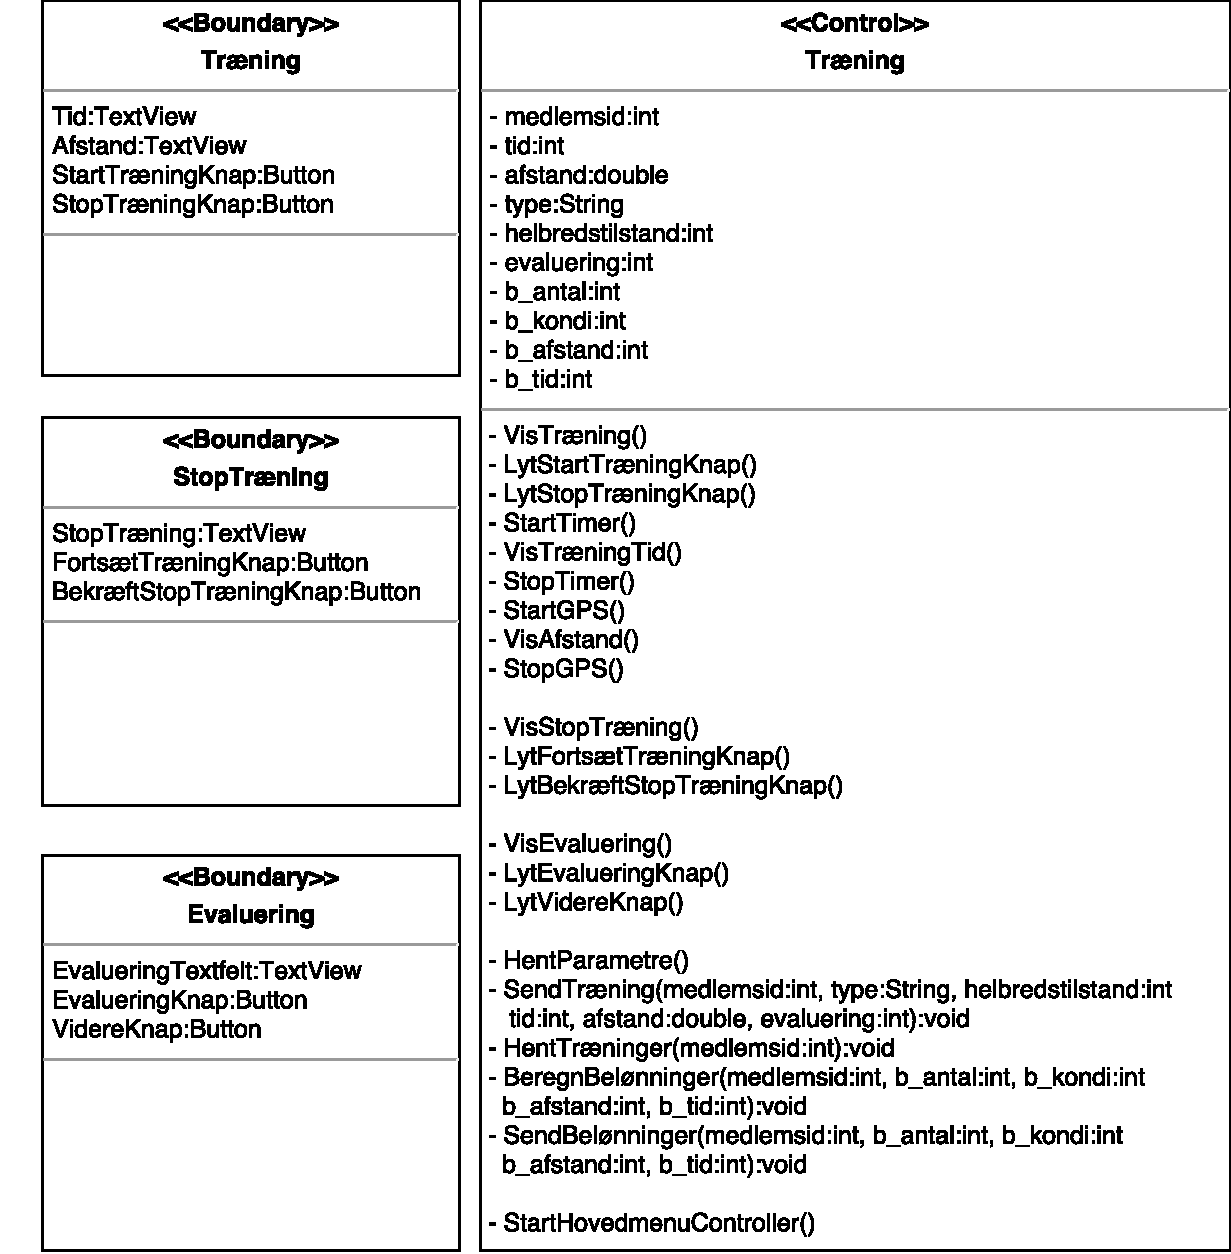
\includegraphics[width=0.9\textwidth]{figures/MVC/MVCTraening}
\caption{Designklasser for træning samt evaluering.}
\label{fig:DesignTraening}
\end{figure}

\textit{TræningGrænsefladen} er den grænseflade, der vises ved en igangværende træning. Denne indeholder tekstfelter, hvori tiden samt afstanden oplyses. Derudover er der et tekstfelt til kompatiblemålinger, hvis disse er tilsluttet. Yderligere indeholder denne grænseflade en stopknap, af typen button, hvis træningen ønskes afsluttet. 
Ønskes træningen afsluttet vises \textit{StopTræningGrænseflade}, hvori der er opstillet et tekstfelt samt to knapper. Tekstfeltet informerer brugeren om, at vedkommende er ved at afslutte træningen, hvorved brugeren kan bekræfte, at træningen skal stoppes eller fortsætte træningen ved hjælp af de opstillede knapper. 
Efter en afsluttet træning, skal træningen evalueres, hvilket forekommer i \textit{EvalueringGrænsefladen}. Denne grænseflade indeholder et tekstfelt, der informerer brugeren om evalueringen, samt fire knapper. De tre knapper er opstillet således brugeren kan evaluere den udførte træning. Evalueringen bekræftes ved, at benytte den sidste knap til at bevæge sig videre i app’en. 
\textit{TræningEvalueringController} er den fælles controller, som bestemmer, hvilken boundary, som vises. Denne controller lagrer tiden, afstanden, evaluering samt kompatible målinger, hvis disse er tilkoblet. Derudover lytter controlleren på de forskellige respektive knapper og håndterer skiftet mellem boundarys. Idet brugeren har evalueret sin træning og bekræftet ved at benytte videreknappen sendes alle træningsoplysningerne til databasen, hvori de gemmes. Dertil returneres brugeren til hovedmenuen. 
